\chapter{Ultracold Fermi Gases}
\label{chapter:ultracold-gases}

In this Chapter, a short introduction to the physics of ultracold Fermi gases is given. First, the concept of Feshbach resonances, which allow to tune the interaction strength inside the gas, and their connection to scattering physics is introduced. Then, the microscopic model and first mean-field descriptions are discussed. For more details, see~\cite{Boettcher2012,Randeria2014,Zwerger2016}.

\section{Feshbach resonances}
\label{section:feshbach-resonances}

In ultracold fermionic gases, the interaction strength can be tuned by means of Feshbach resonances. In order to understand this statement, we have to recover the basic notion of two-body scattering physics at low energies. The relevant parameter, which can be extracted from experiments, is the scattering length $a$. For sufficiently short range interaction potentials, the scattering length describes the scattering process completely. At low temperatures, the s-wave scattering amplitude is given by~\cite{Zwerger2016}
%
\begin{align}
	\label{eq:scattering-amplitude}
	f(k) = \frac{1}{-1/a-ik+\mathcal{O}(k^2)} \,,
\end{align}
%
where $k$ is the center of mass momentum. In real gases, the effective range of interactions is essentially the van der Waals length $l_{\mathrm{vdw}}$ which is much smaller then the average interparticle spacing $n^{-1/3}$ at density $n$. At the same time, the temperature has to be small enough such that the thermal wavelength $\lambda_T$ is larger than the interparticle spacing. Ultracold gases are thus characterized by the following hierarchy of length scales~\cite{Zwerger2016}
%
\begin{align}
	\label{eq:hierarchy-of-scales}
	l_{\mathrm{vdw}} \ll n^{-1/3} \ll \lambda_T \,.
\end{align}
%
The difference between weak and strong interactions is characterized by the relative magnitude of the scattering length with respect to the interparticle distance. Using Feshbach resonances, the scattering length can be tuned to values much larger then the typical interparticle distance while keeping the effective range of order $l_{\mathrm{vdw}}$. In this way, strongly interacting Fermi gases with $n^{-1/3}a\gg 1$ can be realized.

In general, Feshbach resonances can be described with the two-channel model, see Fig.~\ref{fig:feshbach-resonances}. When a bound state in a closed channel is coupled resonantly with the scattering continuum of an open channel, the scattering cross section can be enhanced. Here, one uses the fact that the atoms can virtually change their spin configuration during the collision. In the different spin configuration, they interact with a different scattering potential which can be tuned with a magnetic field $B$ according to the Zeeman splitting $\Delta E=\Delta\mu B$, where $\Delta\mu$ is the difference in magnetic moment between closed and open channel. The energetic distance of the bound state in the closed channel to the scattering threshold $E=0$ is called detuning~\cite{Faigle-Cedzich2022}
%
\begin{align}
	\label{eq:detuning}
	\nu(B) = \Delta\mu (B-B_0) \,,
\end{align}
%
where $B_0$ is the resonance position of the Feshbach resonance, see Fig.~\ref{fig:feshbach-resonances}.

On a phenomenological level, the scattering length can be written as
%
\begin{align}
	\label{eq:scattering-length}
	a(B) = a_{\mathrm{bg}} \left(1-\frac{\Delta B}{B-B_0}\right) \,,
\end{align}
%
where $a_{\mathrm{bg}}$ is a background scattering length without coupling to the closed channel and $\Delta B$ is the width of the resonance. For more discussions about the width $\Delta B$, as well as broad and narrow Feshbach resonances, see e.g.~\cite{Diehl2006-1}. Note that the resonance occurs when the detuning vanishes $\nu(B)\rightarrow 0$. In this case, we are in the so called strongly correlated, unitary regime. To summarize, the following three regimes can be identified in the three-dimensional BCS-BEC crossover, as function of the dimensionless interaction strength $(k_Fa)^{-1}$,
%
\begin{align*}
	(k_F a)^{-1} \rightarrow -\infty \,&: \qquad \text{weakly interacting fermionic gas ,} \\
	|(k_F a)^{-1}| \leq 1 \,&: \qquad \text{strongly interacting regime ,} \\
	(k_F a)^{-1} \rightarrow \infty \,&: \qquad \text{weakly interacting bosonic gas .}
\end{align*}
%
In the following, we are interested in the strongly correlated case close to a broad Feshbach resonance which is described sufficiently by the single-channel model introduced below.


\begin{figure}[t]
	\centering
	\subfigure[]{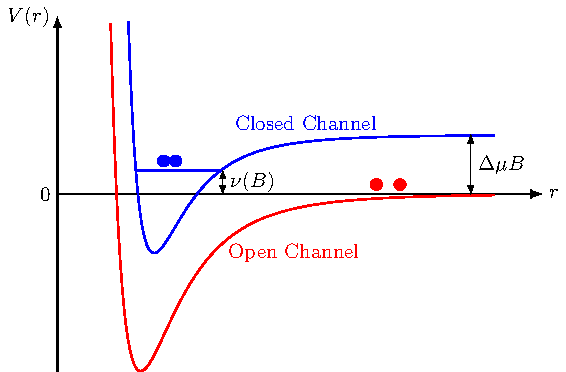
\includegraphics[width=0.49\textwidth]{figs/feshbach.pdf}} 
	\subfigure[]{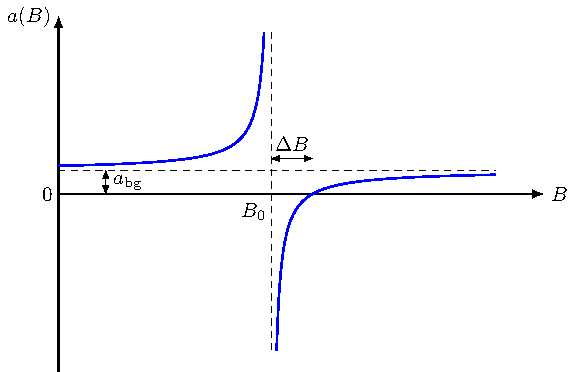
\includegraphics[width=0.49\textwidth]{figs/scattering.pdf}}
	\caption[Feshbach resonance model and scattering length]{(a) Two-channel Feshbach resonance model as described in the main text. (b) Scattering length $a$ as a function of magnetic field $B$, see Eq.~\eqref{eq:scattering-length}.}
	\label{fig:feshbach-resonances}
\end{figure}


\section{Single-channel model}
\label{section:single-channel-model}

We consider a non-relativistic two-component Fermi gas with contact interaction described by the Euclidean action (single-channel model)~\cite{Zwerger2016}
%
\begin{align}
	\label{eq:microscopic-action}
	S[\psi] = \int_{0}^{\beta} d\tau \int d^3 x\,
	\Big[ \sum_{\sigma=\uparrow,\downarrow} \psi_{\sigma}^* (\partial_{\tau} - \nabla^2 - \mu_{\sigma}) \psi_{\sigma}
	+ \lambda \psi_{\uparrow}^*\psi_{\downarrow}^*\psi_{\downarrow}\psi_{\uparrow} \Big] \,,
\end{align}
%
where $\lambda$ is the coupling constant, which is connected to the s-wave scattering length $a$, and $\mu_{\sigma}$ is the chemical potential of fermion species $\sigma = (\uparrow, \downarrow)$.
The fermionic fields $\psi_{\sigma}(\tau,\bm{x})$ are Grassmann valued and depend on the Euclidean time $\tau$, which is restricted to the circumference $\beta=1/T$. Notation and units are as described at the end of the introduction.

Motivated by the Feshbach resonance model, a partially bosonised spin-balanced system ($\mu_{\uparrow}=\mu_{\downarrow}=\mu$) is used, where the contact interaction of fermions is mediated by the exchange of bosonic dimers. Mathematically, this bosonic field enters the microscopic action~\eqref{eq:microscopic-action} via a Hubbard–Stratonovich transformation and the new action is given by
%
\begin{align}
	\label{eq:single-channel-action}
	S[\psi, \phi] = \int_{0}^{\beta} d\tau \int d^3 x\,
	\Big[ \sum_{\sigma=\uparrow,\downarrow} \psi^*_{\sigma} (\partial_{\tau} - \nabla^2 - \mu) \psi_{\sigma}
	+ \nu \phi^* \phi - h (\phi^* \psi_{\uparrow} \psi_{\downarrow} - \phi \psi^*_{\uparrow} \psi^*_{\downarrow}) \Big] \,,
\end{align}
%
where $h$ is the Feshbach coupling between the fermions and bosons, and $\nu$ is the detuning of the dimer. This action is also called single-channel model and is depicted diagrammatically in Fig.~\ref{fig:single-channel-model}. Note that the four-fermion interaction has dropped out, which requires that $\lambda = - h^2 / \nu$~\cite{Floerchinger2009}. Indeed, performing the Gaussian functional integral over the bosonic fields recovers the fermionic action~\eqref{eq:microscopic-action}. This is diagrammatically shown in Fig.~\ref{fig:interaction}. While the four-fermion coupling $\lambda$ gets strongly affected by fluctuations, the Feshbach coupling $h$ which is connected to the width of the resonance can be approximated by its classical value. As a consequence, the bare detuning $\nu$ needs appropriate renormalization, which is described in detail in Appendix~\ref{app:renormalization}. Here, we just state that the bare detuning $\nu$ is related to the two-body scattering length $a$ via~\cite{Diehl2008,Haussmann2007,Frank2018-1}
%
\begin{align}
	\label{eq:renormalized-detuning}
	\nu = -\frac{h^2}{8\pi a} + \int\frac{d^3p}{(2\pi)^3} \frac{1}{2\bm{p}^2} \,.
\end{align}
%
By tuning the dimensionless interaction strength $(k_Fa)^{-1}$, the system can be driven from a BCS-type superfluid to a Bose-Einstein condensed state, allowing for the exploration of the BCS-BEC crossover~\cite{Randeria2014}. On the BCS side of the crossover, $(k_Fa)^{-1}<0$, the bosonic dimer $\phi$ describes weakly bound Cooper pairs. On the BEC side, $(k_Fa)^{-1}>0$, $\phi$ describes tightly bound bosonic molecules. Bose-Einstein condensation of the bosonic pairs, i.e. a non-vanishing expectation value of $\phi$, leads to superfluidity in the system~\cite{SadeMelo1993}. In the following, we will consider the BCS-BEC crossover with a special focus on the strongly correlated, unitary regime at $(k_Fa)^{-1}=0$.

\begin{figure}[t]
	\centering
	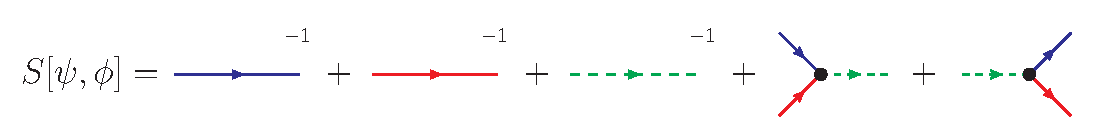
\includegraphics[width=\textwidth]{figs/action.pdf}
	\caption[Single-channel model]{Diagrammatic representation of the single-channel model in Eq.~\eqref{eq:single-channel-action}.
	The two classical fermion propagators are denoted by the blue and red full line, and the classical boson propagator is denoted by the green dashed line.}
	\label{fig:single-channel-model}
\end{figure}


\begin{figure}[b]
	\centering
	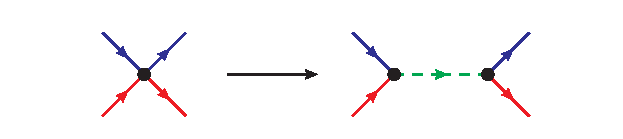
\includegraphics[width=0.6\textwidth]{figs/interaction.pdf}
	\caption[Microscopic interaction]{Diagrammatic representation of the Hubbard-Stratonovich transformation. The four-fermion interaction is modeled by the exchange of a bosonic dimer.}
	\label{fig:interaction}
\end{figure}


\section{Mean-field description} %%% or mean-field theory?
\label{section:nambu-gorkov-formalism}

Before diving into the fully non-perturbative description of the BCS-BEC crossover, it is worth investigating the theory on a mean-field level to get some physical intuition and to introduce the basic notation. In this context, the Nambu-Gorkov formalism~\cite{Boettcher2012} comes in handy, which is also used in other theories of superconductivity~\cite{Strinati2018}. This will also provide us with the mean-field propagators which will be used as initial guess for further computations. Let us define the Nambu spinors in momentum space, with $Q=(\omega_n,\bm{q})$,
%
\begin{align}
	\label{eq:nambu-spinors}
	\Psi^{\dagger}(Q) = \left(\psi_{\uparrow}^*(Q), \, \psi_{\downarrow}(-Q)\right) \,, \quad
	\Psi(Q) = \begin{pmatrix}\psi_{\uparrow}(Q) \\ \psi_{\downarrow}^*(-Q)\end{pmatrix} \,.
\end{align}
%
With these spinors, the fermionic part of the action~\eqref{eq:single-channel-action} can be written as
%
\begin{align}
	\label{eq:fermionic-action}
	S_F[\Psi] = \int_{0}^{\beta} d\tau \int d^3 x\,\, \Psi^{\dagger}
	\begin{pmatrix} \partial_{\tau}-\nabla^2-\mu  & h\phi \\
	h\phi^* & \partial_{\tau}+\nabla^2+\mu \end{pmatrix}
	\Psi \,.
\end{align}
%
From this expression, the inverse classical propagator $S^{(2)}_{\Psi\Psi^{\dagger}}(Q,Q')$
with constant background field $\Delta = h\phi$ can be derived~\cite{Diehl2010}
%
\begin{align}
	\label{eq:fermion-propagator}
	S^{(2)}_{\Psi\Psi^{\dagger}}(Q,Q') = \frac{\delta^2 S_F}{\delta\Psi(Q)\delta\Psi^{\dagger}(Q')} 
	= \delta(Q-Q')
	\begin{pmatrix} -i\omega_n+\varepsilon_{\bm{q}}-\mu & \Delta \\
	\Delta^* & -i\omega_n-\varepsilon_{\bm{q}}+\mu \end{pmatrix} \,,
\end{align}
%
where we defined the classical momentum dispersion $\varepsilon_{\bm{q}}=\bm{q}^2$. The parameter $\Delta$ is often called the gap parameter. A more detailed derivation of the propagators can be found in Appendix~\ref{app:propagators}. Note that a propagator comes always with an energy-momentum conserving delta function $G(Q,Q')=\delta(Q-Q')G(Q)$. In the following, we will call $G(Q)$ the propagator. From Eq.~\eqref{eq:fermion-propagator}, the classical fermion propagator, or BCS propagator, can be obtained via matrix inversion~\cite{VanLoon2020}
\begin{align}
	\label{eq:bcs-propagator}
	G^{(0)}_{\Psi\Psi^{\dagger}}(Q) = \frac{1}{\omega_n^2+\xi_{\bm{q}}^2+\Delta^2}
	\begin{pmatrix} i\omega_n+\xi_{\bm{q}} & \Delta \\
	\Delta^* & i\omega_n-\xi_{\bm{q}} \end{pmatrix} \,,
\end{align}
where $\xi_{\bm{q}}=\varepsilon_{\bm{q}}-\mu$. The components of the BCS propagator can be rewritten in terms of the Bogoliubov coefficients $u_{\bm{q}}, v_{\bm{q}}$ and a new BCS dispersion relation $E_{\bm{q}}=\sqrt{\xi_{\bm{q}}^2+\Delta^2}$,
%
\begin{align}
	\label{eq:bogoliubov-coefficients}
	u_{\bm{q}}^2 = \frac{1}{2}\left[1 + \frac{\xi_{\bm{q}}}{E_{\bm{q}}}\right] \,, \quad
	v_{\bm{q}}^2 = \frac{1}{2}\left[1 - \frac{\xi_{\bm{q}}}{E_{\bm{q}}}\right] \,, \quad
	u_{\bm{q}} v_{\bm{q}} = \frac{\Delta}{2E_{\bm{q}}} \,.
\end{align}
%
We call the diagonal entries of the propagator ($\uparrow\uparrow$, $\downarrow\downarrow$) the normal components,
%
\begin{align}
	\label{eq:normal-components}
	G^{(0)}_{\uparrow\uparrow}(Q) = \frac{i\omega_n+\xi_{\bm{q}}}{\omega_n^2+E_{\bm{q}}^2} = \frac{u_{\bm{q}}^2}{-i\omega_n+E_{\bm{q}}} + \frac{v_{\bm{q}}^2}{-i\omega_n-E_{\bm{q}}}	= - G^{(0)}_{\downarrow\downarrow}(-Q) \,,
\end{align}
%
and the off-diagonal entries ($\uparrow\downarrow$, $\downarrow\uparrow$) the anomalous components,
%
\begin{align}
	\label{eq:anomalous-components}
	G^{(0)}_{\uparrow\downarrow}(Q) = \frac{\Delta}{\omega_n^2+E_{\bm{q}}^2} = u_{\bm{q}} v_{\bm{q}}
	\left[\frac{1}{-i\omega_n+E_{\bm{q}}} - \frac{1}{-i\omega_n-E_{\bm{q}}}\right] = G^{(0)}_{\downarrow\uparrow}(Q) \,.
\end{align}
%
In the last equation, we chose $\Delta$ to be real without loss of generality~\cite{Fetter1971}.

The physical meaning of these components is very intuitive. In the normal phase where there is no condensate, i.e. $\Delta=0$, the off-diagonal components are zero and we are left with a standard fermionic propagator with classical dispersion relation. In the symmetry-broken phase, or superfluid phase, the gap parameter is non-zero ($\Delta\neq 0$) and we obtain a modified BCS dispersion relation, see Fig.~\ref{fig:dispersion-relation}. Thus, the anomalous components are directly related to the presence of a condensate field~\cite{Fetter1971}.

From Eq.~\eqref{eq:normal-components} and~\eqref{eq:anomalous-components}, the general initial spectral functions can be derived,
%
\begin{align}
	\label{eq:initial-spectral-functions}
	\rho^{(0)}_{\uparrow\uparrow}(\lambda,\bm{q}) &= u_{\bm{q}}^2\, \delta(\lambda-E_{\bm{q}}) + v_{\bm{q}}^2\, \delta(\lambda+E_{\bm{q}}) \,, \\
	\rho^{(0)}_{\uparrow\downarrow}(\lambda,\bm{q}) &= u_{\bm{q}} v_{\bm{q}} \left[\delta(\lambda-E_{\bm{q}}) - \delta(\lambda+E_{\bm{q}})\right] \,.
\end{align}
%
In the normal phase ($\Delta=0$), the spectral functions simplify to
%
\begin{align}
	\label{eq:normal-spectral-functions}
	\rho^{(0)}_{\uparrow\uparrow}(\lambda,\bm{q}) &= \delta(\lambda-\bm{q}^2+\mu) \,, \\
	\rho^{(0)}_{\uparrow\downarrow}(\lambda,\bm{q}) &= 0 \,.
\end{align}
%
Since the diagonal components, as well as the off-diagonal components, are related to each other for the spin- and mass-balanced Fermi gas, the system is completely described by one normal and one anomalous spectral function. Note that the anomalous spectral function satisfies the sum rules~\cite{Pieri2004-1}
%
\begin{align}
	\label{eq:anomalous-sum-rules}
	\int_{-\infty}^{\infty} d\lambda\, \rho_{\uparrow\downarrow}(\lambda,\bm{p}) &= 0 \,, \\
	\int_{-\infty}^{\infty} d\lambda\,\lambda\, \rho_{\uparrow\downarrow}(\lambda,\bm{p}) &= \Delta \,.
\end{align}
%
In the single-channel model, the bosonic dimer acts as an interaction exchange particle and has no classical dispersion relation. Thus, it has no clear interpretation as a probability distribution and is not normalized. In this way, it carries also no contribution to the total density. For a more detailed discussion of dynamic bosons within the two-channel model, see~\cite{Diehl2006-1,Diehl2007,Schmidt2013}.


\begin{figure}[b]
	\centering
	\subfigure[]{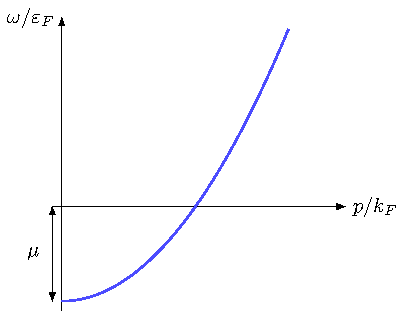
\includegraphics[width=0.42\textwidth]{figs/dispersion1.pdf}} 
	\subfigure[]{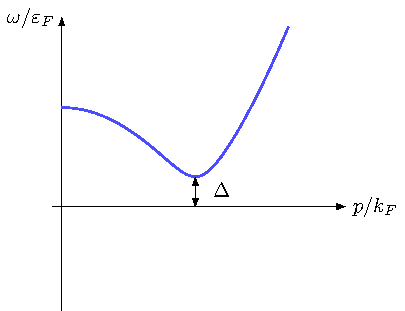
\includegraphics[width=0.42\textwidth]{figs/dispersion2.pdf}}
	\caption[Dispersion relations]{(a) Classical dispersion relation in the normal phase vs. (b) BCS dispersion relation in the superfluid phase.}
	\label{fig:dispersion-relation}
\end{figure}